\documentclass[10pt,a4paper,twocolumn]{article}

\usepackage[czech]{babel}
\usepackage[utf8]{inputenc}
\usepackage[T1]{fontenc}
\usepackage{graphicx}
\usepackage{float}
\usepackage{amsmath}
\usepackage{hyperref}
\usepackage{caption}
\usepackage{titlesec}
\usepackage{geometry}
\geometry{margin=1.5cm}
\usepackage{makecell}
\renewcommand\theadalign{bc}
\renewcommand\theadfont{\bfseries}
\renewcommand\theadgape{\Gape[1pt]}

\titleformat{\section}{\large\bfseries}{\thesection}{1em}{}
\titleformat{\subsection}{\normalsize\bfseries}{\thesubsection}{1em}{}

\title{\textbf{Závěrečná zpráva - Raytracer s akcelerační strukturou}}
\author{Jakub Votrubec \\
ČVUT FIT, NI-PG1 2024/25}
\date{}

\begin{document}

\maketitle

%================================================================================

\section{Úvod}
Tento dokument popisuje závěrečný výstup, v podobě semestrální práce, z předmětu NI-PG1. Náplní semestrální práce bylo vytvoření vlastního raytracering renderu a implementace akcelerační datové struktury pro zrychlení traverzace scény. Cílem bylo prokázat schopnost optimalizovat výkon raytraceru pomocí vhodné datové struktury.
Semestrální práce byla zpracována v jazyce C++, standard C++17, a využívá externí knihovny pouze pro načítání scén a konfigurace ve formátu \texttt{json}.

%================================================================================

\section{Struktura raytraceru}

Implementoval jsem základní raytracer pro vykreslování scén složených z trojúhelníků. Raytracer má následující funkce, mezi kterými lze přepínat pomocí konfigurace:

\begin{itemize}
    \item Stíny pomocí stínových paprsků.
    \item Podpora plošného světla skrze náhodné vzorkování trojúhelníků.
    \item Vykreslení scény s různými osvětlovacími modely (distance shading, čistě difuzní osvětlení, Phongův osvětlovací model, Blinn-Phongův osvětlovací model).
    \item Vykreslení scény s různými stánovacími modely (flat shading, smooth shading - Phongův stínovací model).
    \item Podpora odrazu a lomu světla.
    \item Backface culling.
    \item Vykreslení scény s více vzorky na pixel (fuzzysampling), viz \textit{Použité metody nad rámec cvičení}.
\end{itemize}

Raytracer je navržen tak, aby byl modulární a snadno rozšiřitelný. Hlavní třída \texttt{Raytracer} obsahuje metody pro vykreslování a ukládání výsledného obrazu. Scéna je reprezentována jako seznam trojúhelníků, které jsou načteny z~\texttt{.obj} souboru.

Raytracer načítá scénu pomocí knihovny \texttt{tinyobjloader} a používá knihovnu \texttt{nlohmann/json} pro načítání konfigurace. Scéna se vykreslí do formátu~\texttt{.ppm}.

\subsection{Použité metody nad rámec cvičení}

Při renderování scény jsem zjistil problém s velkým množstvím šumu ve výsledném obrazu. Rozhodl jsem se implementovat několikanásobné vzorkování. Metodu jsem nazval \textit{fuzzysampling}.

\textit{Fuzzysampling} spočívá v tom, že pro každý pixel se vygeneruje několik paprsků, ale každý s lehce pozměněným směrem paprsku. Jejich výsledky se poté průměrují. Tím se dosáhne hladšího obrazu a sníží se šum. Zmeny směru paprsk jsou generovány náhodně v rámci pixelu, což umožňuje zachovat detaily a zároveň eliminovat šum.

%================================================================================

\section{Akcelerační datová struktura}

Implemetoval jsem dvě varianty akcelerační datové struktury octree:
\begin{itemize}
    \item základní varianta octree,
    \item parametrická varianta podle článku \textit{An Efficient Parametric Algorithm for Octree Traversal} od Revelles et al..
\end{itemize}

\subsection{Stavba a traverzace}

Octree je struktura, která dělí prostor na menší buňky, což umožňuje rychlejší vyhledávání kolizí mezi paprsky a trojúhelníky. Každý uzel octree obsahuje bounding box, který definuje prostor, který uzel pokrývá, a seznam trojúhelníků, které se v tomto prostoru nacházejí.

\subsubsection{Základní octree}

Základní octree je implementován jako rekurzivní struktura, která dělí prostor rekurzivně na osm dalších uzlů (oktetů), dokud není dosaženo maximální hloubky nebo počtu trojúhelníků v uzlu.

Traverzace probíhá tak, že pro každý paprsek se nejprve zjistí, zda protíná bounding box aktuálního uzlu. Pokud ano, poračuje se dál na jeho oktety, pokud ne, traverzace končí. Je-li oktet již list stromu (neobsahuje žádné vlastní oktety), traverzace končí a jeho trojúhelníky jsou přidány k výsledku. Traverzace pokračuje rekurzivně, dokud se neprohledá celý strom. Prochází se vždy všechny oktety uzlu.

\subsubsection{Parametrický octree}

Parametrický octree je vylepšená verze, která využívá parametrickou traverzaci. Tato metoda umožňuje efektivnější prohledávání prostoru tím, že využívá parametrické rovnice pro určení průsečíků paprsku s hranicemi uzlů octree (tzv. "slab" metoda).

Nejprve se vypočítájí průsečíky paprsku s~hranicemi uzlu, z~nich se určtí "čas", kdy paprsek vstoupí a~opustí daný uzel na jednotlivých osách. Pokud paprsek opustil uzel na nějaké ose dříve, nežli vstoupil na všech osách - minul bounding box uzlu a tato větev traverzace se ozavírá.

Pokud paprsek vstoupil, tak na základě průsečíku vstupu se vypočítá první oktet, do kterého paprsek vstoupí. Ten se následně přidá do fronty pro další zpracování. Následně se postupně se projdou a přidají všechny oktety, do kterých paprsek vstoupí. Procházení všech dalších oktetů probíhá na základě konečného automatu, který určuje, do kterého oktetu paprsek vstoupí na základě jeho směru a aktuálního oktetu.

Optimalizace oproti základnímu octree spočívá v~tom, že se neprocházejí všechny oktety, ale pouze ty, do kterých paprsek skutečně vstoupí. Zároveň výpočet velikostí oktetů je založen jen na půlení velikosti rodičovského uzlu, což umožňuje efektivní a~výpočetně nenáročné dělení prostoru.

Parametrickou traverzaci se mi bohužel nepodařilo implementovat, vice viz \textit{Problémy při implementaci}.

\subsection{Problémy při implementaci}

Při implementaci stavby octree jsem narazil na problémy s~přesností výpočtů velikosti oktetů. Kvůli chybě u datových typů s plovoucí desteinou čárkou se ne vždy přiřadily všechny trojúhelníky rodičovského uzlu do jeho oktetů, což vedlo k~chybám při traverzaci. Tento problém jsem vyřešil nafouknutím bounding boxů o toleranci \textit{epsilon}.

Bohužel se  mi nepodařilo správně implementovat a zprovoznit parametrický octree. Narazil na problémy při traverzaci. Traverzace nenalezne všechny trojúhelníky a scéna je poté vyrenderována s dírami, jak švýcarský sýr. Zkoušel jsem, jestli je problém opět v přesnosti výpočtů s čísly s plovoucí desetinnou čárkou, ale nepodařilo se mi ho vyřešit. Proto jsem se rozhodl parametrický octree nevyužít a~v~měření výkonu použít pouze základní octree.

%================================================================================

\section{Měření výkonu}

\subsection{Nastavení měření}

Pro měření výkonu byla použita scéna \texttt{CornellBox-Sphere.obj} s následující konfigurací:

\begin{table}[H]
    \centering
    \caption{Použité nastavení rendereru}
    \begin{tabular}{|l|l|}
        \hline
        \thead{Parametr} & \thead{Hodnota} \\
        \hline
        Výsledné rozlišení & $800 \times 800$ \\
        \hline
        Max. zanoření paprsku & 10 \\
        \hline
        \makecell{Vzorků plošného světla \\ na trojúhelník} & 50 \\
        \hline
        Osvětlovací model & Blinn-Phong \\
        \hline
        Stínovací model & Smooth \\
        \hline
        Backface culling & Ano \\
        \hline
        Fuzzysampling & Ne \\
        \hline
    \end{tabular}
\end{table}

\begin{table}[H]
    \centering
    \caption{Použité nastavení struktury octree}
    \begin{tabular}{|l|c|}
        \hline
        \thead{Parametr} & \thead{Hodnota} \\
        \hline
        Max. počet trojúhelníků na uzel & 16 \\
        \hline
        Max. hloubka uzlů & 10 \\
        \hline
    \end{tabular}
\end{table}

\subsection{Výsledky měření}

Porovnání výkonu bez akcelerační struktury a s akcelerační strukturou octree:

\begin{table}[H]
    \centering
    \caption{Porovnání výkonu raytraceru}
    \begin{tabular}{|l|c|c|}
        \hline
        \thead{Metrika} & \thead{Bez ADS} & \thead{Octree} \\
        \hline
        Čas renderování [s] & 3h 24m 12.4s & 13m 53.7s \\
        \hline
        \makecell{Počet kolizí \\ paprsek-trojúhelník} & $2.46 \times 10^{11}$ & $2.81 \times 10^{9}$ \\
        \hline
        \makecell{Průměrný počet kolizí \\ na paprsek} & 383\,665 & 4\,395 \\
        \hline
        Čas výpočtu kolizí [s] & 8\,032.8 & 121.5 \\
        \hline
        \makecell{Průměrná doba výpočtu \\ kolizí na paprsek [ms]} & 12.55 & 0.19 \\
        \hline
    \end{tabular}
\end{table}

\begin{table}[H]
    \centering
    \caption{Statistiky struktury octree}
    \begin{tabular}{|l|c|}
        \hline
        \thead{Statistika} & \thead{Hodnota} \\
        \hline
        Počet uzlů & 1\,584 \\
        \hline
        Počet listů & 1\,300 \\
        \hline
        Průměrná hloubka listů & 5.22 \\
        \hline
        Max. trojúhelníků v listu & 34 \\
        \hline
        Průměr trojúhelníků v listu & 7.03 \\
        \hline
        Čas stavby octree [s] & 0.04 \\
        \hline
        Počet prohledaných uzlů & 1\,138\,825\,603 \\
        \hline
        Čas strávený traverzací & 4m 43.943s \\
        \hline
        \makecell{Průměrný počet trojúhelníků \\ vrácených z traverzace} & 33.7 \\
        \hline
    \end{tabular}
\end{table}

%================================================================================

\section{Ukázky výstupů}

\begin{figure}[H]
    \centering
    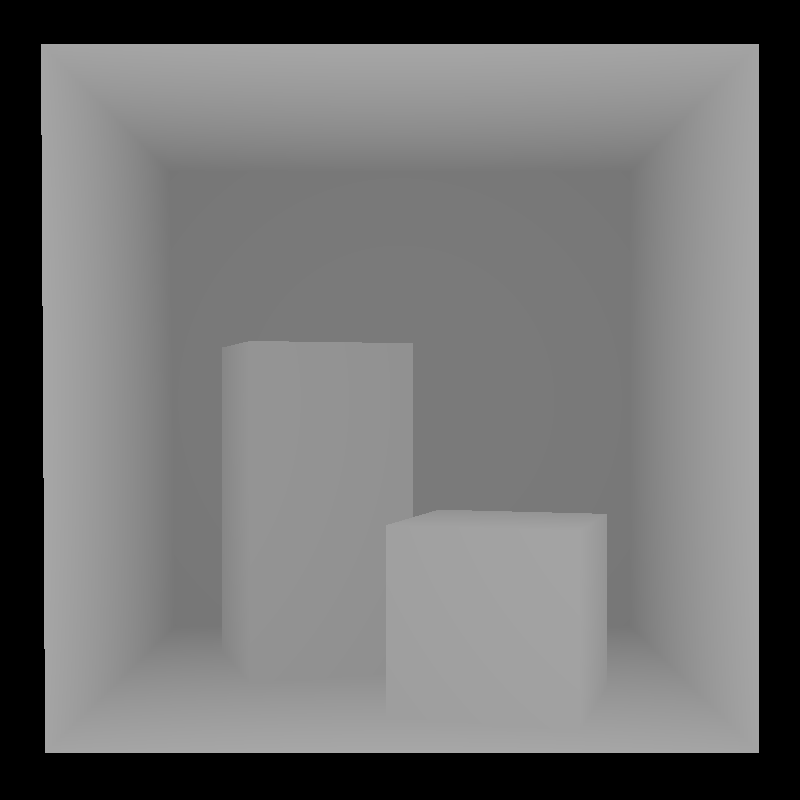
\includegraphics[width=0.38\textwidth]{images/box_render_distance.png}
    \caption{Ukázka vykreslení scény s distance shadingem.}
\end{figure}

\begin{figure}[H]
    \centering
    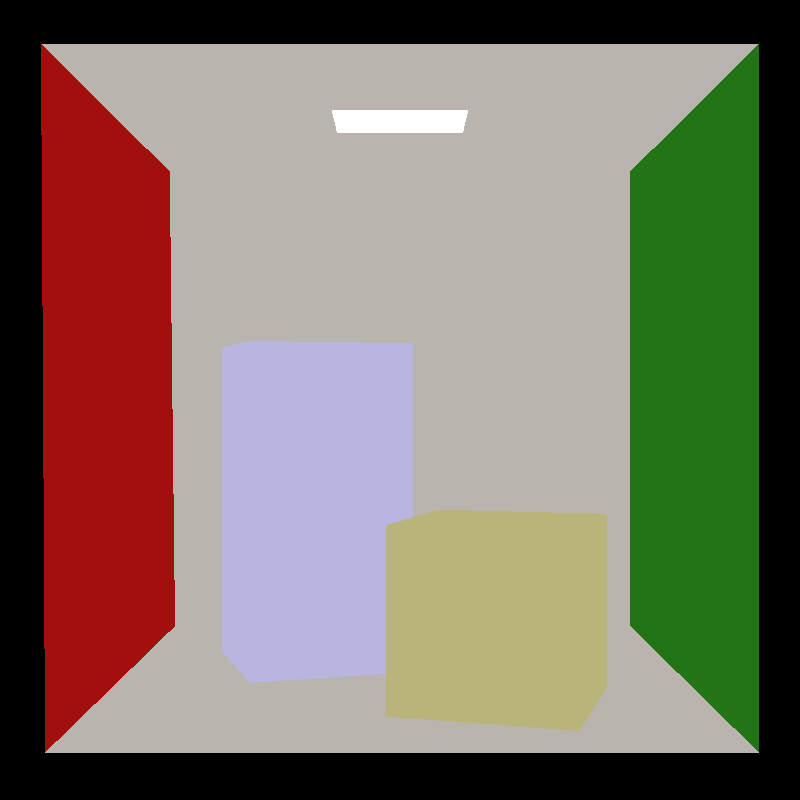
\includegraphics[width=0.38\textwidth]{images/box_render_diffusion.png}
    \caption{Ukázka vykreslení scény s difúzním osvětlením.}
\end{figure}

\begin{figure}[H]
    \centering
    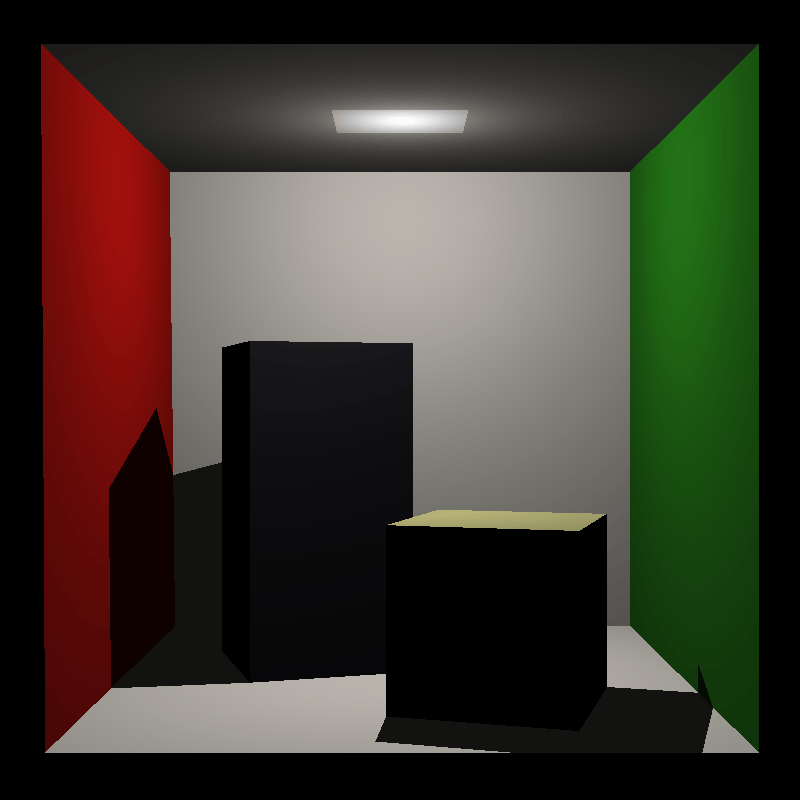
\includegraphics[width=0.38\textwidth]{images/box_render_blinn-phong_shadows.png}
    \caption{Ukázka vykreslení scény s Blinn-Phong osvětlením a stíny.}
\end{figure}

\begin{figure}[H]
    \centering
    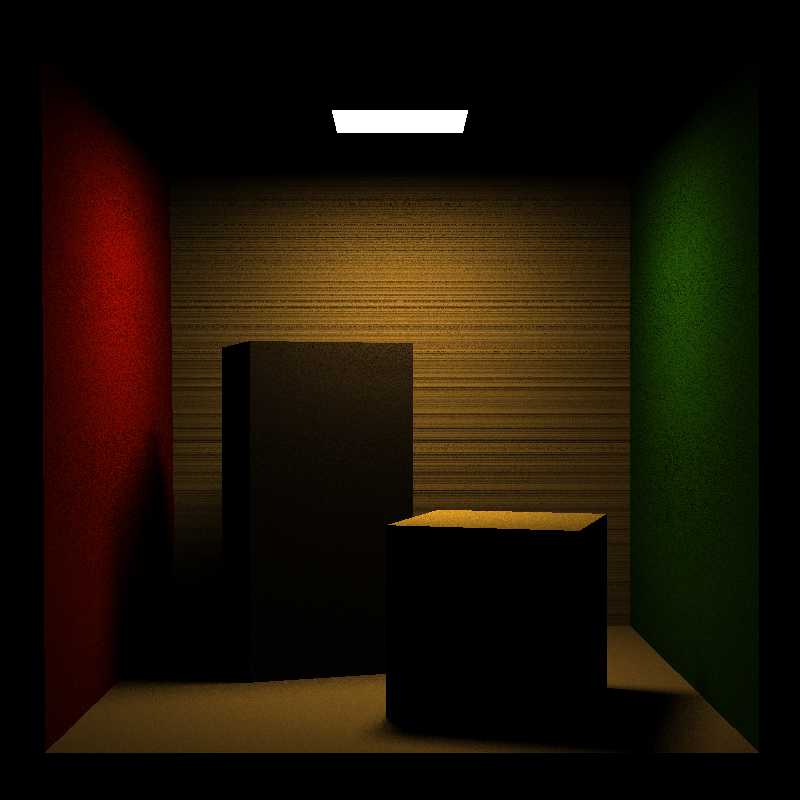
\includegraphics[width=0.38\textwidth]{images/box_render_area_lights.png}
    \caption{Ukázka vykreslení scény s plošným světlem.}
\end{figure}

\begin{figure}[H]
    \centering
    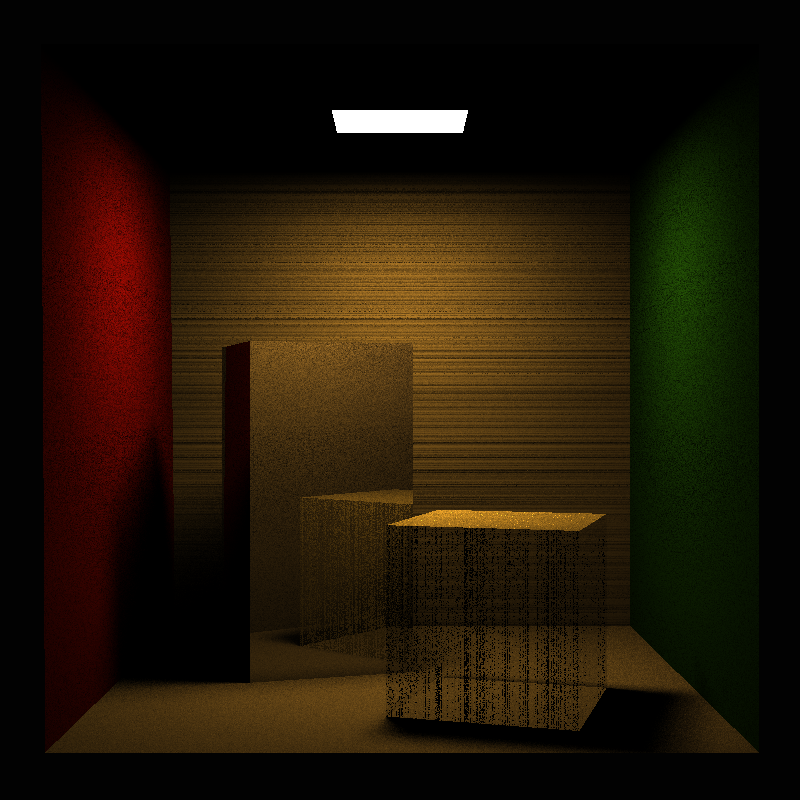
\includegraphics[width=0.38\textwidth]{images/box_render_reflection_refraction.png}
    \caption{Ukázka vykreslení scény s odrazem a lomem světla.}
\end{figure}

\begin{figure}[H]
    \centering
    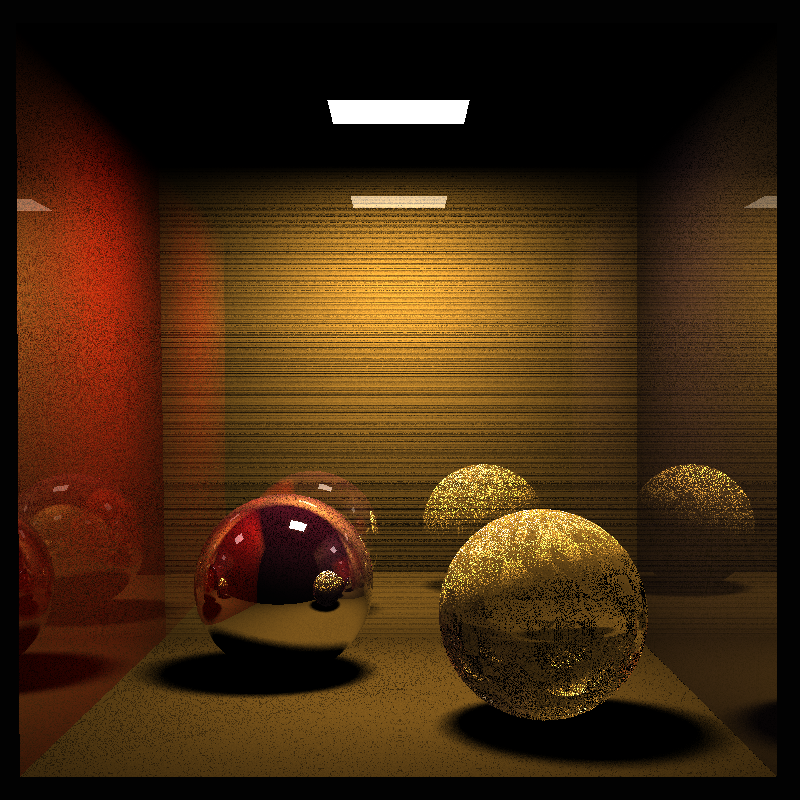
\includegraphics[width=0.38\textwidth]{images/sphere_render_reflection_refraction_walls.png}
    \caption{Ukázka vykreslení scény s odrazem a lomem světla na zrcadlových stěnách.}
\end{figure}

\begin{figure}[H]
    \centering
    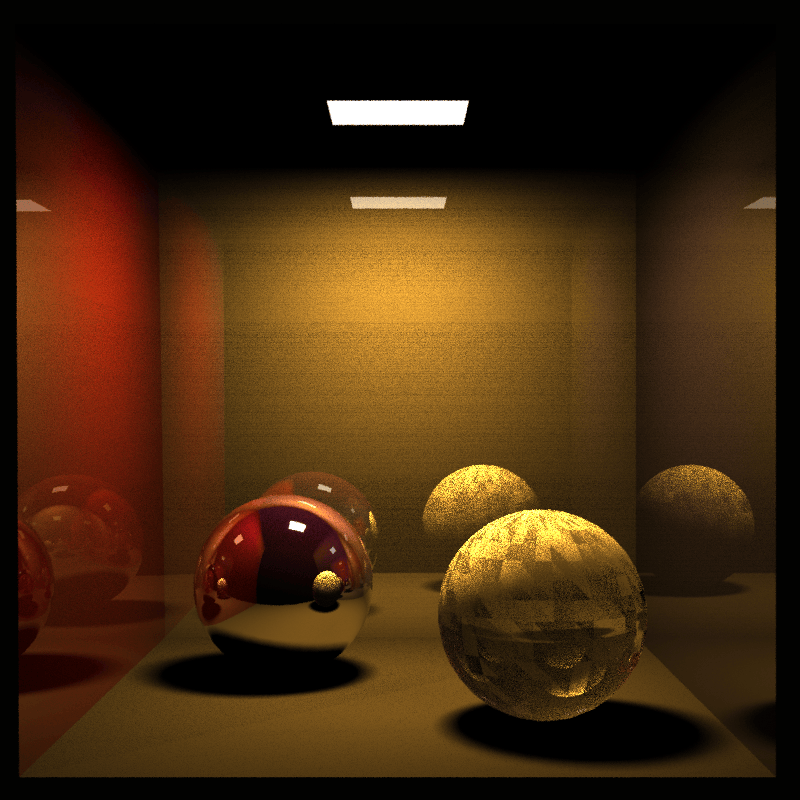
\includegraphics[width=0.38\textwidth]{images/sphere_render_sampling_10.png}
    \caption{Ukázka vykreslení scény s fuzzysamplingem (10~vzorků na pixel).}
\end{figure}

%================================================================================

\section{Implementace}

Veškerá implementace je dostupná na fakultním \href{https://gitlab.fit.cvut.cz/votruja6/pg1-raytracer#}{GitLabu} a mém \href{https://github.com/MasterVotr/PG1-raytracer}{GitHubu}.

Více informací o kompilaci, konfiguraci a spuštění naleznete v~souboru README samotného repozitáře.

%================================================================================

\section{Závěr}

Tato semestrální práce prokázala schopnost optimalizovat výkon raytraceru pomocí akcelerační datové struktury octree. Implementace základního octree vedla k~významnému zrychlení traverzace scény a~snížení počtu kolizí mezi paprsky a~trojúhelníky. Parametrickou variantu octree se mi bohužel nepodařilo implementovat, což je škoda, protože by mohla přinést další zlepšení výkonu.

Další rozšíření raytraceru by mohlo zahrnovat implementaci dalších akceleračních struktur, jako jsou BVH (Bounding Volume Hierarchy) nebo kd-stromy, které by mohly dále zlepšit výkon při renderování složitějších scén.

Rád bych také zkusil implementovat paralelní zpracování raytraceru, což by mohlo výrazně zrychlit renderování na moderních vícejádrových procesorech nebo GPU.

\section{Použitá literatura}
\begin{itemize}
    \item Přednášky a materiály z předmětu NI-PG1.
    \item \textit{An Efficient Parametric Algorithm for Octree Traversal} - Revelles et al.
    \item \texttt{tinyobjloader} - Knihovna pro načítání \texttt{.obj} souborů.
    \item \texttt{nlohmann/json} - Knihovna pro práci s~JSON v~C++.
    \item Dokumentace k C++ standardu a knihovnám.
\end{itemize}


\end{document}
